\subsection{Fuentes de Información}\label{fuentes-de-informaciuxf3n}

Una fuente de información se define como una tupla \((\mathcal{S},P)\)
donde

\begin{itemize}
\tightlist
\item
  \(\mathcal{S}\) es un conjunto de símbolos que pueden ser emitidos por
  la fuente (un alfabeto).
\item
  \(P\) es una distribución de probabilidades asociada (a la emisión) de
  lo los símbolos.
\end{itemize}

Las fuentes de información pueden ser contínuas (con un número de
mensajes no numerable) o discretas (con un número de mensajes numerable
o finito). En este curso nos centraremos en el caso discreto, por ende
\(S\) será un conjunto finito.

Claramente, \(\forall s\in\mathcal{S}, 0\leq P(s)\leq 1\), y
\(\sum_{s \in\mathcal{S}} P(s) = 1\) (debido a los Axiomas de
Kolmogorov).

\subsubsection{Fuentes de Información de Memoria
Nula}\label{fuentes-de-informaciuxf3n-de-memoria-nula}

En una fuente de información de memoria nula, la emisión de cada símbolo
\(s_i\) es independiente de los símbolos emitidos anteriormente. En este
caso, la probabilidad de emitir un símbolo \(s_i\) es constante e igual
a \(P(s_i)\).

La entropía de una fuente de información de memoria nula se define como

\[
H(\mathcal{S}) = -\sum_{s\in\mathcal{S}} P(s)\log\left(P(s)\right)
\]

\subsubsection{\texorpdfstring{Extensión de grado
\(m\)}{Extensión de grado m}}\label{extensiuxf3n-de-grado-m}

Podemos imaginarnos la fuente de información de memoria nula como una
máquina que emite secuencias de \(x\) símbolos, palabras,
\(x\in\mathcal{S}^+\), de modo que los símbolos sucesivamente emitidos
se eligen de acuerdo con las probabilidades \(P(s)\).

Sea entonces \(|x|=m\), definimos la extensión de grado \(m\) de la
fuente de información de memoria nula como el par
\(\left(\mathcal{S}^m, P^m\right)\), donde

\[
\forall x\in\mathcal{S}^m:P(x)=\prod_{1\leq i\leq m}P(x[i])
\]

Y trivialmente, la entropía


\begin{align*}
H\left(\mathcal{S}^m\right)&=-\sum_{x\in\mathcal{S}^m}P(x)\log\left(P(x)\right)\\
&=-\sum_{x\in\mathcal{S}^m}\left(\prod_{1\leq i\leq m}P(x[i])\right)\log\left(P(\prod_{1\leq i\leq m}P(x[i]))\right)
\end{align*}


En lugar de calcular los productos de probabilidades de los símbolos
para cada una de las palabras de la extensión de grado \(m\), se puede
demostrar el siguiente útil resultado:

\[
H\left(\mathcal{S}^m\right)=mH(\mathcal{S})
\]

\subsubsection{\texorpdfstring{Fuentes de Markov (fuente de información
con memoria, de orden
\(m\))}{Fuentes de Markov (fuente de información con memoria, de orden m)}}\label{fuentes-de-markov-fuente-de-informaciuxf3n-con-memoria-de-orden-m}

En una fuente de Markov, la emisión de cada símbolo \(s_i\) depende de
los \(m\) símbolos emitidos anteriormente (en muchas aplicaciones). En
este caso, la probabilidad de emitir un símbolo \(s_i\) depende de los
\(m\) símbolos anteriores, y se denota como la probabilidad condicional
\(P(s_i|s_{i-1},\ldots,s_{i-m})\), con

\[
\sum_{i=1}^{m}P(s_i|s_{i_1},\ldots,s_{i_m})= 1,\quad i_k = 1,2,\dots,n
\]

A la secuencia de símbolos emitidos se les llama \textbf{cadena de
Markov}. Los estados de una fuente de Markov (de orden \(m\)) serán
todas las posibles combinaciones de \(m\) símbolos \(n^m\).

Dada una fuente de Markov de orden \(m\), se puede establecer su
diagrama de estados que muestra los estados y las probabilidades entre
ellos.

\begin{center}\rule{0.5\linewidth}{0.5pt}\end{center}

\paragraph{Ejemplos}\label{ejemplos}

A partir de un alfabeto binario \(\left\{0,1\right\}\), se puede definir
una fuente de Markov de orden 2 con los siguientes estados y
probabilidades condicionales:

\begin{itemize}
\tightlist
\item
  \(P(0|00)=P(1|11)=0.7\)
\item
  \(P(1|00)=P(0|11)=0.3\)
\item
  \(P(0|01)=P(1|10)=P(0|10)=P(1|01)=0.5\)
\end{itemize}

\pagebreak

El diagrama de estados es el siguiente:

\begin{figure}[htbp!]
\centering
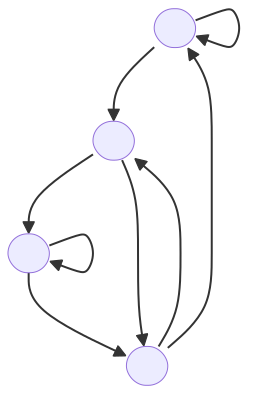
\includegraphics[width=0.5\linewidth]{./img/fuente-de-markov-diagrama-de-estados.png}
\end{figure}

\begin{center}\rule{0.5\linewidth}{0.5pt}\end{center}

Se dice que una fuente de Markov es ergódica si es posible pasar de
cualquier estado a cualquier otro estado en un número finito de pasos.

\begin{center}\rule{0.5\linewidth}{0.5pt}\end{center}

\paragraph{Ejemplo}\label{ejemplo}

Una fuente ergódica podría ser la anterior (podemos alcanzar cualquier
estado en un número finito de pasos a partir de otro estado).

Ejemplo de diagrama de estados de una fuente ergódica:

\begin{figure}[htbp!]
\centering
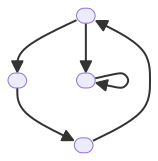
\includegraphics[width=0.25\linewidth]{./img/fuente-de-markov-no-ergódico.png}
\end{figure}

Nótese que el nodo interior es un estado absorbente. Es decir, una vez
que se llega a ese estado, no se puede salir de él.

\begin{center}\rule{0.5\linewidth}{0.5pt}\end{center}

Una fuente de Markov es homogénea si las probabilidades condicionales no
cambian con el tiempo.

Se dice que una fuente está en estado estacionario si la probabilidad de
observación de sus estados no cambia con el tiempo. Las probabilidades
se pueden obtener mediante la ecuación \(v=\pi\Pi\), donde \(\pi\) es el
vector de probabilidad de los estados y \(\Pi\) es la matriz de
transición.

\begin{center}\rule{0.5\linewidth}{0.5pt}\end{center}

\paragraph{Ejemplo}\label{ejemplo-1}

Volviendo al ejemplo inicial, la matriz de probabilidades tiene la
siguiente forma:

\[
\Pi = \begin{matrix}
& \begin{matrix} 00 & 01 & 10 & 11 \end{matrix} \\
\begin{matrix} 00 \\ 01 \\ 10 \\ 11 \end{matrix} & \begin{pmatrix} 0.7 & 0.5 & 0.5 & 0.3 \\ 0.5 & 0.5 & 0.5 & 0.5 \\ 0.5 & 0.5 & 0.5 & 0.5 \\ 0.3 & 0.5 & 0.5 & 0.7 \end{pmatrix}
\end{matrix}
\]

Véase que cada fila suma 1 (debido a los axiomas de Kolmogorov). Si cada
columna sumase 1, entonces la matriz es doblemente estocástica y todos
los estados son equiprobables.

Vayamos al cálculo de probabilidades de estados en régimen estacionario.
Para ello, nos definimos las siguientes ecuaciones:


\begin{align*}
&P(00) = P(0|00)\cdot P(00) + P(0|10)\cdot P(10)\\
&P(01) = P(1|00)\cdot P(00) + P(0|10)\cdot P(10)\\
&P(11) = P(1|01)\cdot P(01) + P(1|11)\cdot P(11)\\
&P(00) + P(01) + P(10) + P(11) = 1
\end{align*}


Nótese que la última ecuación surge por uno de los axiomas de
Kolmogorov, ya que si incluyésemos el estado \(01\) en la primera
ecuación, tendríamos una ecuación redundante (y por ende un sistema
singular; con infinitas soluciones). Conocemos las probabilidades
condicionaes, por lo que podemos resolver el sistema de ecuaciones:


\begin{align*}
&P(00) = 0.7\cdot P(00) + 0.5\cdot P(10)\\
&P(01) = 0.3\cdot P(00) + 0.5\cdot P(10)\\
&P(11) = 0.5\cdot P(01) + 0.7\cdot P(11)\\
&P(00) + P(01) + P(10) + P(11) = 1
\end{align*}


Este sistema tiene la siguiente solución:

\[
\pi = \begin{pmatrix} P(00) \\ P(01) \\ P(10) \\ P(11) \end{pmatrix} = \begin{pmatrix} \frac{5}{16} \\ \frac{3}{16} \\ \frac{3}{16} \\ \frac{5}{16} \end{pmatrix}
\]

Ahora, con esta información podemos calcular las probabilidades de
aparición de cada símbolo:


\begin{align*}
&P(0) = P(00) + P(10) = \frac{5}{16} + \frac{3}{16} = \frac{8}{16} = \frac{1}{2}\\
&P(1) = P(01) + P(11) = \frac{3}{16} + \frac{5}{16} = \frac{8}{16} = \frac{1}{2}
\end{align*}


\begin{center}\rule{0.5\linewidth}{0.5pt}\end{center}

\subsubsection{Fuentes afines (adjuntas) de una fuente de
Markov}\label{fuentes-afines-adjuntas-de-una-fuente-de-markov}

Dada una fuente de Markov de orden \(m\) con un alfabeto \(\mathcal{S}\)
y una distribución de probabilidad \(P\), denominaremos a la fuente afín
como a la fuente de memoria nula \((\mathcal{S},P)\). Es decir, la
fuente afín es la fuente de memoria nula que emite los mismos símbolos
que la fuente de Markov.

\begin{center}\rule{0.5\linewidth}{0.5pt}\end{center}

\paragraph{Ejemplo}\label{ejemplo-2}

Para el ejemplo de la fuente de Markov de orden 2, la fuente afín sería
la fuente de memoria nula con \(\mathcal{S}=\left\{0,1\right\}\) y
\(P=\left\{\frac{1}{2},\frac{1}{2}\right\}\).

\begin{center}\rule{0.5\linewidth}{0.5pt}\end{center}

Para el cálculo de entropía de una fuente de Markov de orden \(m\),
sobre un alfabeto \(\mathcal{S}=\left\{s_1,s_2,\dots,s_n\right\}\) y
distribución de probabilidad condicional
\(P(s_i|s_{i_1},\dots,s_{i_m})\), se cumple que
\(p(s_i, s_{i_1},\dots,s_{i_m}) = p(s_i|s_{i_1},\dots,s_{i_m})\cdot p(s_{i_1},\dots,s_{i_m})\),
lo cual nos permite calcular la entropía condicional:

\[
H(\mathcal{S}|s_{i_1},\dots,s_{i_m}) = -\sum_{i=1}^{n}p(s_i|s_{i_1},\dots,s_{i_m})\log\left(p(s_i|s_{i_1},\dots,s_{i_m})\right)
\]

Por lo tanto, la entropía de la fuente de Markov de orden \(m\) es:


\begin{align*}
H(\mathcal{S}) &= \sum_{\mathcal{S}^m}p(s_{i_1},\dots,s_{i_m})H(\mathcal{S}|s_{i_1},\dots,s_{i_m})\\
&= -\sum_{\mathcal{S}^m}p(s_{i_1},\dots,s_{i_m})\left(-\sum_{s_i\in\mathcal{S}}p(s_i|s_{i_1},\dots,s_{i_m})\log\left(p(s_i|s_{i_1},\dots,s_{i_m})\right)\right)\\
&= -\sum_{\mathcal{S}^{m+1}}p(s_i, s_{i_1},\dots,s_{i_m})p(s_i|s_{i_1},\dots,s_{i_m})\log\left(p(s_i|s_{i_1},\dots,s_{i_m})\right)\\
&= -\sum_{\mathcal{S}^{m+1}}p(s_{i_1},\dots,s_{i_m},s_i)\log\left(p(s_i|s_{i_1},\dots,s_{i_m})\right)\\
\end{align*}

